\documentclass[11pt]{beamer}
\usetheme{Goettingen}
\usepackage[utf8]{inputenc}
\usepackage{amsmath}
\usepackage{amsfonts}
\usepackage{amssymb}
\usepackage{graphicx}
\usepackage{hyperref}
\author{Alex Heilman}
\title{Quantum Teleportation}
\subtitle{No-cloning and a simple example}
%\setbeamercovered{transparent} 
%\setbeamertemplate{navigation symbols}{} 
%\logo{} 
%\institute{} 
%\date{} 
%\subject{} 

\newenvironment{boxed2}
    {\begin{center}
    \begin{tabular}{|p{0.95\textwidth}|}
    \hline\\
    }
    { 
    \\\\\hline
    \end{tabular} 
    \end{center}
    }


\begin{document}

\begin{frame}
\titlepage
\end{frame}

%\begin{frame}
%\tableofcontents
%\end{frame}

\begin{frame}{Overview}

$\bullet$ Quantum No-Cloning

\vspace{1cm}\pause

$\bullet$ Quantum Teleportation \pause (Two-Party, Qubit State) 

\vspace{1cm}\pause

$\bullet$ Experimental Setup


\end{frame}

\section{No-Cloning}
\begin{frame}{No-Cloning}

\begin{boxed2}
\textbf{Quantum No-Cloning Theorem:} The quantum no-cloning theorem states that arbitrary, unknown quantum states cannot be cloned/replicated.
\end{boxed2}\pause

More formally, there is no unitary (linear) transformation $U$ that can evolve a secondary state such that some other, arbitrary state is replicated, as below:

$$
\vert \psi\rangle \otimes \vert 0\rangle \rightarrow\vert \psi\rangle \otimes \vert \psi \rangle  
$$ \pause
\begin{center}
\textbf{NOT ALLOWED!!!}
\end{center}
\end{frame}

\begin{frame}{No-Cloning: Simple Proof}
Consider the following action of a 'copy' on the basis states:
\begin{align*}
\vert 0 \rangle & \rightarrow \vert 0 \rangle\otimes \vert 0 \rangle=\vert 00\rangle\\
\vert 1 \rangle & \rightarrow \vert 1 \rangle\otimes \vert 1 \rangle = \vert 11\rangle
\end{align*}\pause

Now, let's define $\vert \phi \rangle = \vert 0\rangle+\vert 1 \rangle$:\pause
\begin{align*}
\vert \phi \rangle & \rightarrow \vert \phi \rangle\otimes \vert \phi \rangle\\
& = \big( \vert 0\rangle+\vert 1 \rangle \big)\otimes \big( \vert 0\rangle+\vert 1 \rangle \big)\\
& = \vert 00\rangle + \vert 01\rangle +\vert 10\rangle +\vert 11\rangle
\end{align*}\pause
But, due to the linearity of the transformation we should also have:

\vspace{-.4cm}

\begin{align*}
\vert 0\rangle+\vert 1 \rangle & \rightarrow \vert 00\rangle  +\vert 11\rangle
\end{align*}
\begin{center}\small\pause
\textbf{CONTRADICTION!}
\end{center}

\end{frame}

\begin{frame}{No-Cloning cont.}
Of course, this proof relies on the assumption that we are dealing only with pure states and that the form of the cloning algorithm/evolution is unitary. \pause

\vspace{1cm}

A more general theorem that extends to mixed states and quantum operations is known as the quantum no-broadcasting theorem.
\end{frame}

\section{Teleportation}
\begin{frame}{Quantum Teleportation}
Let's assume a simple two-party system in which the parties are spatially distant and would like to transmit or 'teleport' a qubit state to one another.

\vspace{0.7cm}

\begin{center}
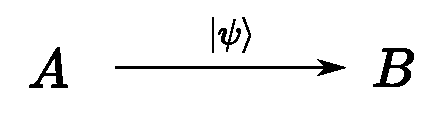
\includegraphics[scale=0.7]{teleschematic.pdf}
\end{center}

\vspace{0.7cm}\pause

Often times, party one is termed Alice (A) and party two is termed Bob (B)
\end{frame}

\begin{frame}{Teleportation: Step-by-Step}
For such a two-party system the teleportation scheme is as below:\pause

\vspace{.5cm}

\begin{itemize}
\item[1]Distribute entangled qubit pair between parties \pause

\item[2]Evolve entangled qubit locally with arbitrary state
\begin{itemize}
\item[a] Apply CNOT Gate
\item[b] Apply Hadamard Gate
\end{itemize}\pause
\item[3]Measure local state after evolution\pause
\item[4]Transmit (classical) measurement result to other party\pause
\item[5]Evolve local state of other party's entangled qubit dependent on measurement result\pause
\end{itemize}

\vspace{.5cm}
\begin{center}
State is now 'teleported'!
\end{center}

\end{frame}

\begin{frame}{{\small ASIDE:} Causality}
Causality refers to the concept of cause and effect; according to Einstein's relativity, nothing can travel faster than light.\pause

\vspace{1cm}

Effectively, we shouldn't be able to communicate any information faster than the speed of light or causality is said to be violated. \pause

\vspace{1cm}

The necessary transmission of the (classical) information describing the measurement outcome of party A guarantees that causality is preserved.
\end{frame}

\begin{frame}{Teleportation 1}
Alice begins with state $\vert\psi\rangle = \alpha \vert 0\rangle + \beta\vert 1 \rangle$ and receives one half of the entangled Bell pair $\vert +\rangle=\big(\vert 00\rangle + \vert 11\rangle\big)/\sqrt{2}$

\vspace{0.5cm}

\begin{center}
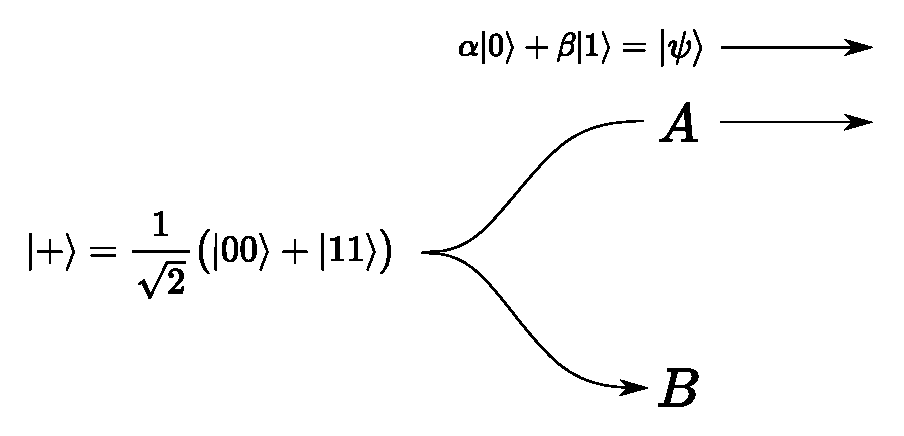
\includegraphics[scale=0.6]{tele1.pdf}
$$
\frac{1}{\sqrt{2}}\big[ \alpha(\vert 000\rangle+\vert 011\rangle) + \beta (\vert 100\rangle + \vert 111\rangle) \big]
$$
\end{center}

\end{frame}


\begin{frame}{Teleportation 2 (a)}
Alice applies a controlled $X$ gate on her qubit state (as control) and her half of the entangled pair (as target)

\vspace{0.5cm}

\begin{center}
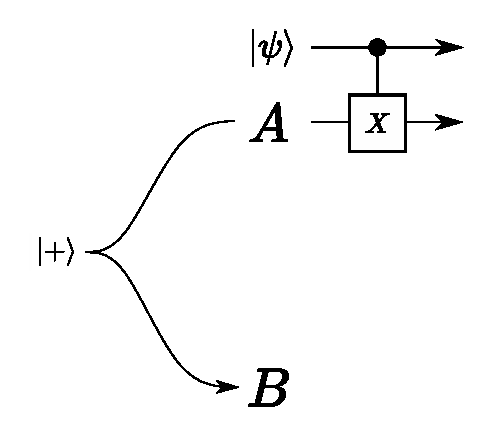
\includegraphics[scale=0.6]{tele2.pdf}
$$
\frac{1}{\sqrt{2}}\big[ \alpha(\vert 000\rangle+\vert 011\rangle) + \beta (\vert 101\rangle + \vert 110\rangle) \big]
$$
\end{center}
\end{frame}

\begin{frame}{Teleportation 2 (b)}
Alice then applies a Hadamard ($H$) gate on her qubit state 

\vspace{0.5cm}

\begin{center}
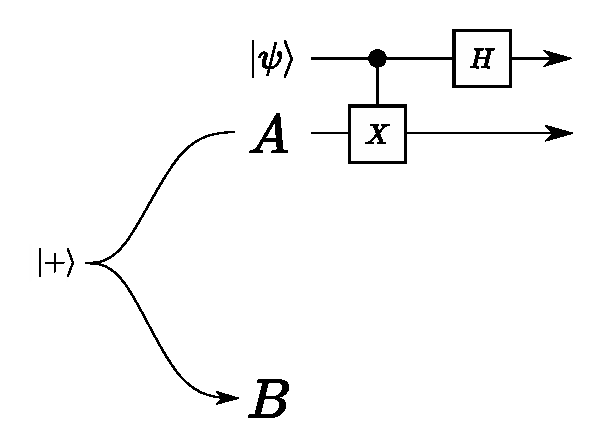
\includegraphics[scale=0.6]{tele3.pdf}
\begin{align*}
\frac{1}{2}\big[& \alpha(\vert 000\rangle+\vert 011\rangle+\vert 100\rangle+\vert 111\rangle) \\
+& \beta (\vert 001\rangle + \vert 010\rangle-\vert 101\rangle - \vert 110\rangle) \big]
\end{align*}
\end{center}
\end{frame}

\begin{frame}{Teleportation 3}
Alice then measures her qubit and her half of the entangled qubit

\vspace{0.5cm}

\begin{center}
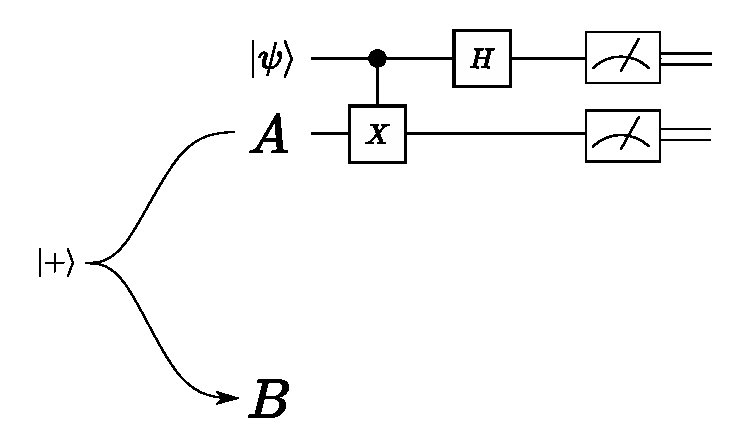
\includegraphics[scale=0.7]{tele4.pdf}

\end{center}
\end{frame}


\begin{frame}{Teleportation 4}\small
Recall that the total state before measurement is proportional to the following:
\begin{align*}
& \alpha(\vert 000\rangle+\vert 011\rangle+\vert 100\rangle+\vert 111\rangle) \\
+& \beta (\vert 001\rangle + \vert 010\rangle-\vert 101\rangle - \vert 110\rangle)
\end{align*}
\pause

Let's now consider what such measurement results tell us about the resulting state (which Bob is in possession of):

\begin{align*}
\text{A measures } \ \vert 00\rangle\rightarrow\quad & \alpha \vert 0 \rangle+\beta \vert 1 \rangle = \vert \psi \rangle\\
\vert 01\rangle\rightarrow \quad & \alpha \vert 1 \rangle+\beta \vert 0 \rangle =X \vert \psi \rangle\\
\vert 10\rangle\rightarrow \quad & \alpha \vert 0 \rangle - \beta \vert 1\rangle= Z \vert \psi \rangle \\
\vert 11\rangle\rightarrow \quad & \alpha \vert 1 \rangle - \beta \vert 0\rangle = XZ \vert \psi \rangle\\
\end{align*}\pause
So, Alice may transmit her measurement results (classically) to Bob, and he will know exactly what state he has with regards to Alice's arbitrary initial state. 
\end{frame}

\begin{frame}{Teleportation 5}
Bob then tailors his gate application according to Alice's results:
\pause

\begin{align*}
\text{A sends result } \ \vert 00\rangle\rightarrow\quad & \alpha \vert 0 \rangle+\beta \vert 1 \rangle \ \  \text{Bob applies nothing}\\
\vert 01\rangle\rightarrow \quad & \alpha \vert 1 \rangle+\beta \vert 0 \rangle \ \  \text{Bob applies } X\\
\vert 10\rangle\rightarrow \quad & \alpha \vert 0 \rangle - \beta \vert 1\rangle \ \  \text{Bob applies } Z \\
\vert 11\rangle\rightarrow \quad & \alpha \vert 1 \rangle - \beta \vert 0\rangle  \ \  \text{Bob applies } XZ\\
\end{align*}

\pause
Bob is then guaranteed to have the qubit state $\vert \psi \rangle$!
\end{frame}

\begin{frame}{Notes on Teleportation}\small
Note that Alice's state has been destroyed but she has effectively transmitted it or 'teleported' it to Bob. In fact, Alice may not even know the state of her qubit, $\vert \psi\rangle$.

\pause

\vspace{.45cm}

Quantum teleportation is beneficial (as opposed to simply transmitting the qubit state itself) in certain circumstances for several reasons:

\pause

\medskip

$\bullet$ The classical communication channel may be faster and more reliable

\medskip\pause

$\bullet$ Transmitting unknown quantum states isn't as reliable

\medskip\pause

$\bullet$ Can pre-disperse entangled states to transmit quantum information later

\vspace{.45cm}\pause

Hence, quantum teleportation can help reduce computational errors, be used to construct more resilient quantum networks, and form secure communication channels. May be the foundation of any 
future 'quantum internet'!

\end{frame}

\section{Experiment}
\begin{frame}{Recent experiment}
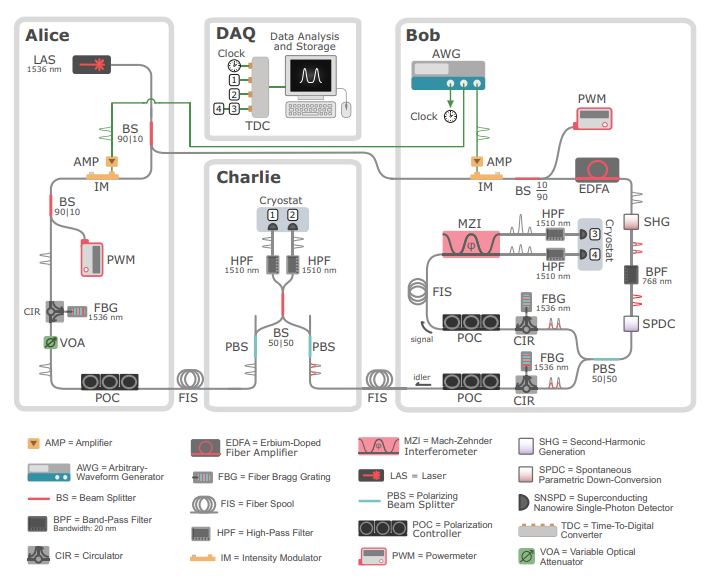
\includegraphics[scale=0.5]{experiment.png}\cite{PRXQuantum.1.020317}

\end{frame}

\section*{Recap}
\begin{frame}{Recap}
Arbitrary, unknown quantum states cannot be unambiguously 'cloned' or copied

\vspace{.5cm}\pause

Such quantum states can be 'teleported' however by means of distributed entangled pairs and classical information transmission

\vspace{.5cm}\pause

Such schemes may be the foundation for future quantum networks
\end{frame}

\begin{frame}{Next time?}

\begin{center}
Any ideas? \pause Thanks for your time!
\end{center}

\end{frame}

\begin{frame}[allowframebreaks]{References}
\bibliographystyle{plain}

\bibliography{qtele} 

\end{frame}
\end{document}